%ustawienia
\documentclass[12pt,a4paper]{article}
\usepackage[T1]{fontenc}
\usepackage{mathptmx}
\usepackage[utf8]{inputenc}
\usepackage{amssymb}
\usepackage[polish]{babel}
\usepackage{polski}
\usepackage{amsmath}
\usepackage{amsfonts}
\usepackage[left=3.5cm,right=2cm,top=2.5cm,bottom=2.5cm]{geometry}
\usepackage{graphicx}
\usepackage{indentfirst} 
\usepackage{float}
\usepackage{hyperref}
\usepackage[most]{tcolorbox}
\usepackage{fancyhdr}
\setlength{\parindent}{0.7cm}
\hypersetup{
	colorlinks = true,
	linkcolor = black,
	filecolor = magenta,
	urlcolor = blue,
	}
\urlstyle{same}	
	
\author{
	\\\includegraphics[width=0.7\linewidth]{img/logoPWSZ.eps} \\\\
	\hfill Karpiński Maciej\\
	\hfill Krysa Marcin\\
	\hfill Kuczma Łukasz\\
	\hfill Mertuszka Adam\\\\	
	\hfill Prowadzący mgr inż. Marcin Tracz
	}
\title{\textbf{Programowanie urządzeń mobilnych}\\\line(1,0){400}\\\textbf{laboratorium}}
\date{}

\begin{document}

	%Stron tytułowa
	\maketitle
	\thispagestyle{fancy}
	\fancyhf{}
	\rhead{\textcolor{gray}{\footnotesize Państwowa Wyższa Szkoła Zawodowa im. Witelona w Legnicy\\Informatyka, rok IV\\Semestr zimowy 2021/2022}}	
	\renewcommand{\headrulewidth}{0pt}
	\clearpage

	%Spis treści
	\pagestyle{fancy}
	\rfoot{\thepage}	
	\tableofcontents
	\newpage

	%Krótki opis projektu
	\section{Projekt}	
	
\includegraphics[]{img/logo.png}
	\\\\
	\indent HotScrew jest mobilną aplikacją, umożliwiającą robotom znalezienie swojej drugiej połówki i umówienie się z nią na randkę przy pomocy wbudowanego czatu.
	Wzorem przy projektowaniu i programowaniu była aplikacja Tinder.
	HotScrew dostępna jest na smartphony z~systemem operacyjnym Android. Zastosowana technologia umożliwia przy niewielkiej modyfikacji zbudowanie działającej
	aplikacji na smartphony z systemem iOS lub aplikacji webowej.\\
	\indent Makiety interfejsu aplikacji został zaprojektowane w aplikacji Figma.
	\begin{center}
		
\includegraphics[width=0.6\linewidth]{img/Welcome.png}
		
\includegraphics[width=0.6\linewidth]{img/Register.png}
		
\includegraphics[width=0.6\linewidth]{img/Login.png}
		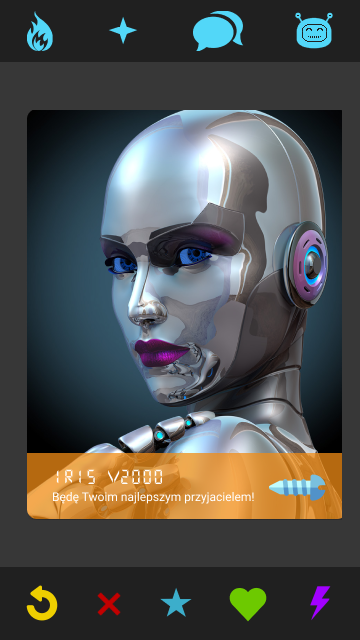
\includegraphics[width=0.6\linewidth]{img/Android1.png}
		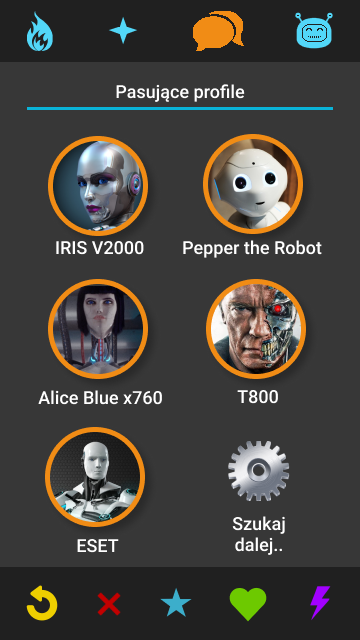
\includegraphics[width=0.6\linewidth]{img/Android2.png}
	\end{center}
	Projekt makiet znajduje się pod adresem: \\ \url{https://www.figma.com/proto/TK3rKQmCnMuTWLookJ7uWl/HotScrew}\\
	Repozytorium projektu znajduje się pod adresem: \\ \url{https://github.com/MacKarp/HotScrew}
		\newpage
	\section{Podział prac}
	\indent Nad projektem aplikacji pracowała czteroosobowa grupa. Skład i podział prac wyglądał następująco:
	\begin{enumerate}
		\item Karpiński Maciej:
			\begin{itemize}
				\item Project Manager
				\item DevOps;
				\item Implementacja backendu aplikacji;
				\item Backend AWS Amplify.
			\end{itemize}
		\item Krysa Marcin:
			\begin{itemize}
				\item Backend AWS Amplify;
				\item Implementacja backendu aplikacji;
				\item Implementacja czatu.
			\end{itemize}
		\item Kuczma Łukasz:
			\begin{itemize}
				\item Projekt graficzny makiet;
				\item System dopasowań;
				\item Implementacja frontendu aplikacji.
			\end{itemize}
		\item Mertuszka Adam:
			\begin{itemize}
				\item Implementacja frontendu aplikacji;
				\item Implementacja czatu.
				\item System dopasowań.
			\end{itemize}	
	\end{enumerate}
		\newpage
	\section{Opis funkcjonalny systemu}	
	\indent Aplikacja HotScrew realizuje następne funkcjonalności:
	\begin{itemize}
		\item Rejestracja i logowanie przy pomocy e-maila;
		\item Logowanie przy pomocy konta Facebooka;
		\item Logowanie przy pomocy konta Google;
		\item Personalizacja profilu;
		\item Przeglądanie dopasowanych profilów;
		\item Polubienie i odrzucenie profilu;
		\item Czat między dopasowanymi profilami;
		\item Obsługa AWS Amplify;
		\item Aplikacja działająca na systemie operacyjnym Android.
	\end{itemize}
		\newpage
	\section{Opis technologiczny}
	\indent Aplikacja HotScrew została stworzona przy wykorzystaniu następującej technologii:
		\subsection{Amazon Cognito Identity SDK for JavaScript}
			\indent Pakiet Amazon Cognito Identity SDK dla JavaScript umożliwia aplikacjom obsługującym JavaScript rejestrowanie i uwierzytelnianie użytkowników a także przeglądanie,
			usuwanie i aktualizowanie atrybutów użytkowników w ramach usługi Amazon Cognito Identity. Posiada również funkcje zmiany haseł dla uwierzytelnionych użytkowników
			oraz zmianę zapomnianych haseł dla nieuwierzytelnionych	użytkowników. Użytkownicy mogą korzystać z~wielu funkcji bezpieczeństwa, w tym opartego na SMS-ach
			i weryfikacji konta przez telefon lub e-mail. Funkcje hasła wykorzystują protokół Secure Remote Password, aby uniknąć przesyłania haseł w postaci zwykłego tekstu przez sieć.
		\subsection{Android Studio}
			\indent Android Studio jest oficjalnym zintegrowanym środowiskiem programistycznym dla systemu operacyjnego Android firmy Google, zbudowane na bazie oprogramowania IntelliJ IDEA
			firmy JetBrains i zaprojektowane specjalnie z myślą o programowaniu aplikacji na Androida. Jest dostępny do pobrania dla systemów operacyjnych Windows, macOS i Linux.
		\subsection{AWS Amplify}
			\indent AWS Amplify to zestaw specjalnie zaprojektowanych narzędzi i funkcji, które pozwalają programistom frontendowym i mobilnym szybko i łatwo tworzyć aplikacje
			z pełnym stosem na AWS, z elastycznością pozwalającą na wykorzystanie szerokiego zakresu usług AWS w miarę ewolucji przypadków użycia.
			Przy wykorzystaniu Amplify można skonfigurować backend aplikacji internetowej lub mobilnej, podłączyć aplikację w kilka minut, wizualnie zbudować interfejs użytkownika
			internetowego i łatwo zarządzać zawartością aplikacji poza konsolą AWS.
		\subsection{AWS Amplify React Native}
			\indent AWS Amplify React Native to biblioteka JavaScript dla programistów frontendowych i~mobilnych tworzących aplikacje działające w chmurze. Biblioteka zapewnia
		deklaratywny i łatwy w użyciu interfejs w różnych kategoriach operacji w chmurze. AWS Amplify dobrze współpracuje z dowolnym przepływem pracy frontendu opartym
		na JavaScript i React Native.
		\subsection{Core Asynciterator Polyfill}
			\indent Biblioteka zapewnia obsłguę dla Symbol.asyncIterator dla platform, które domyślnie go nie obsługują. Importowanie tej biblioteki umożliwia korzystanie iteratora
		asynchronicznego i może być używany np. w pętli for await...of.
		\subsection{Expo}
			\indent Expo to framework i platforma dla uniwersalnych aplikacji React. Jest zestawem narzędzi i usług zbudowanych na platformach React Native i natywnych, które pomagają
		tworzyć, budować, wdrażać i szybko iterować na iOS, Androidzie i aplikacjach internetowych z tej samej bazy kodu JavaScript/TypeScript.
		\subsection{Expo AV}
			\indent Moduł frameworku Expo zapewniający odtwarzanie Audio i Wideo.
		\subsection{Expo ImagePicker}
			\indent Moduł frameworku Expo zapewniający dostęp do interfejsu użytkownika systemu w~celu wybierania zdjęć i filmów z biblioteki telefonu lub robienia zdjęć aparatem.
		\subsection{Expo Linking}
		\indent Moduł frameworku Expo zapewnia narzędzia do interakcji aplikacji z innymi zainstalowanymi aplikacjami za pomocą precyzyjnych linków. Udostępnia również metody
		pomocnicze do konstruowania i analizowania precyzyjnych linków do aplikacji.
		\subsection{Expo React Native ActionSheet}
			ActionSheet to wieloplatformowy komponent React Native, który korzysta z natywnego UIActionSheet w systemie iOS i implementacji JS w systemie Android.
		\subsection{Feather icons}
			\indent Paczka ikon na licencji open source.
		\subsection{InAppBrowser for React Native}
			\indent Biblioteka InAppBrowser for React Native zapewnia dostęp do przeglądarki internetowej systemu i obsługuje obsługę przekierowań. Niestandardowe karty Chrome
			na Androida i Safari oraz usługę uwierzytelniania na iOS.
		\subsection{Node.js}
			\indent Node.js to otwarte, wieloplatformowe środowisko wykonawcze JavaScript, które działa na silniku V8 i wykonuje kod JavaScript poza przeglądarką internetową.
			Node.js pozwala programistom używać JavaScript do pisania narzędzi wiersza poleceń oraz do wykonywania skryptów po stronie serwera w celu tworzenia dynamicznej
			zawartości strony internetowej przed jej wysłaniem do przeglądarki internetowej użytkownika. Node.js reprezentuje paradygmat „JavaScript wszędzie”, ujednolicając
			tworzenie aplikacji internetowych wokół jednego języka programowania, zamiast różnych języków dla skryptów po stronie serwera i~klienta.
			Node.js ma architekturę sterowaną zdarzeniami zdolną do asynchronicznego we/wy. Te wybory projektowe mają na celu optymalizację przepustowości i~skalowalności
			w~aplikacjach internetowych z wieloma operacjami wejścia/wyjścia, a także w aplikacjach internetowych czasu rzeczywistego (np. programy do komunikacji w~czasie
			rzeczywistym i~gry przeglądarkowe).
		\subsection{NPM}
			\indent NPM to menedżer pakietów dla języka programowania JavaScript. Jest domyślnym menedżerem dla środowiska wykonawczego JavaScript Node.js. Składa się z klienta
			wiersza poleceń, zwanego również npm, oraz internetowej bazy danych publicznych i płatnych pakietów prywatnych, zwanej rejestrem npm.
			Dostęp do rejestru uzyskuje się za pośrednictwem klienta, a dostępne pakiety można przeglądać i przeszukiwać za pośrednictwem strony npm.
			Menedżerem pakietów i rejestrem zarządza npm, Inc.
		\subsection{React}
			\indent React to javascriptowa biblioteka służąca do budowania interfejsów użytkownika. Została zaprojektowana z myślą o stopniowym wdrażaniu.
			Dzięki temu zawarte w niej rozwiązania możesz stosować wybiórczo w zależności od potrzeb.
		\subsection{React Native}
			\indent React Native to platforma oprogramowania interfejsu użytkownika typu open source stworzona przez Meta Platforms, Inc. Służy do tworzenia aplikacji
			na systemy Android, Android TV, iOS, macOS, tvOS, Web, Windows i UWP, umożliwiając programistom korzystanie z Framework React wraz z natywnymi możliwościami
			platformy. Jest również używany do tworzenia aplikacji wirtualnej rzeczywistości w firmie Oculus.
		\subsection{React Native Async Storage}
			\indent Asynchroniczny, niezaszyfrowany, trwały system przechowywania danych typu klucz-wartość dla React Native.
		\subsection{React Native Community}
			\indent Biblioteka rozszerzająca możliwości React Native stworzona przez użytkowników skupionych wokół projektu React Native.
		\subsection{React Native Emoji Selector}
			\indent Biblioteka React Native dodająca element interfejsu wybierania ikon emoji. 
		\subsection{React Native Gesture Handler}
			\indent React Native Gesture Handler zapewnia oparte na natywnym interfejsie API zarządzanie gestami w celu tworzenia najlepszych możliwych
			doświadczeń dotykowych w React Native. Dzięki tej bibliotece gesty nie są już kontrolowane przez system odpowiedzi JS, ale zamiast tego są rozpoznawane i śledzone
			w wątku interfejsu użytkownika. Dzięki temu interakcje dotykowe i śledzenie gestów są nie tylko płynne, ale także niezawodne i deterministyczne.
		\subsection{React Native Image Picker}
			\indent Moduł React Native, który pozwala wybrać zdjęcie lub wideo z biblioteki urządzenia albo aparatu. 
		\subsection{React Native Permissions}
			\indent Moduł React Native zapewniający zunifikowany interfejs API uprawnień dla React Native na iOS, Android i Windows.
		\subsection{React Native Picker}
			\indent React Native Picker jest komponentem bibliotecznym, który pozwala zaprojektować wielokrotny wybór z pisaniem bardzo małej ilości kodu. Jest to menu rozwijane lub
			okno dialogowe, w których użytkownicy mogą wybrać jeden z elementów listy z opcji.
		\subsection{React Native Picker Select}
			\indent Komponent Picker dla React Native, który emuluje natywne interfejsy <select> dla iOS i Android.
		\subsection{React Native Reanimated}
			\indent React Native Reanimated zapewnia wszechstronną bibliotekę animacji, dzięki czemu pozwala na znacznie większą elastyczność, szczególnie
			jeśli chodzi o interakcje oparte na gestach.
		\subsection{React Native SafeAreaContext}
			\indent React Native SafeAreaContext zapewnia elastyczny interfejs API do uzyskiwania dostępu do informacji o bezpiecznym obszarze urządzenia.
			Pozwala to na odpowiednie umieszczenie treści wokół wycięć, pasków stanu, wskaźników domu i innych podobnych elementów interfejsu urządzenia i systemu operacyjnego.
			Zapewnia również komponent SafeAreaView, którego można użyć zamiast View, aby automatycznie wstawić widoki w celu uwzględnienia bezpiecznych obszarów.
		\subsection{React Native VectorIcons}
			\indent Paczka ikon na licencji open source.
		\subsection{uuidv4}
			\indent Biblioteka umożliwiająca w prosty sposób wygenerowanie UUID v4.
		\subsection{Visual Studio Code}
			\indent Visual Studio Code – darmowy edytor kodu  źródłowego z kolorowaniem składni dla wielu języków, stworzony przez Microsoft, o otwartym kodzie  źródłowym.
			Oprogramowanie ma wsparcie dla debugowania kodu, zarządzania wersjami kodu  źródłowego za pośrednictwem systemu kontroli wersji Git,
			automatycznego uzupełniania kodu IntelliSense, zarządzania wycinkami kodu oraz jego refaktoryzacji. Funkcjonalność aplikacji można rozbudować za pomocą rozszerzeń
			instalowanych z dedykowanego repozytorium. Według badania przeprowadzonego przez serwis StackOverflow w 2018 roku, Visual Studio Code zostało ogłoszone
			najpopularniejszym narzędziem służącym wytwarzaniu oprogramowania, za którym na drugim miejscu znajduje się produkt tego samego twórcy, Microsoft Visual Studio.
			Oprogramowanie zostało stworzone w oparciu o framework Electron.
	\newpage
	\section{Interfejs aplikacji}
	\indent Interfejs aplikacji wygląda następująco:
	\begin{center}
		
\includegraphics[width=0.6\linewidth]{img/int1.jpg}
		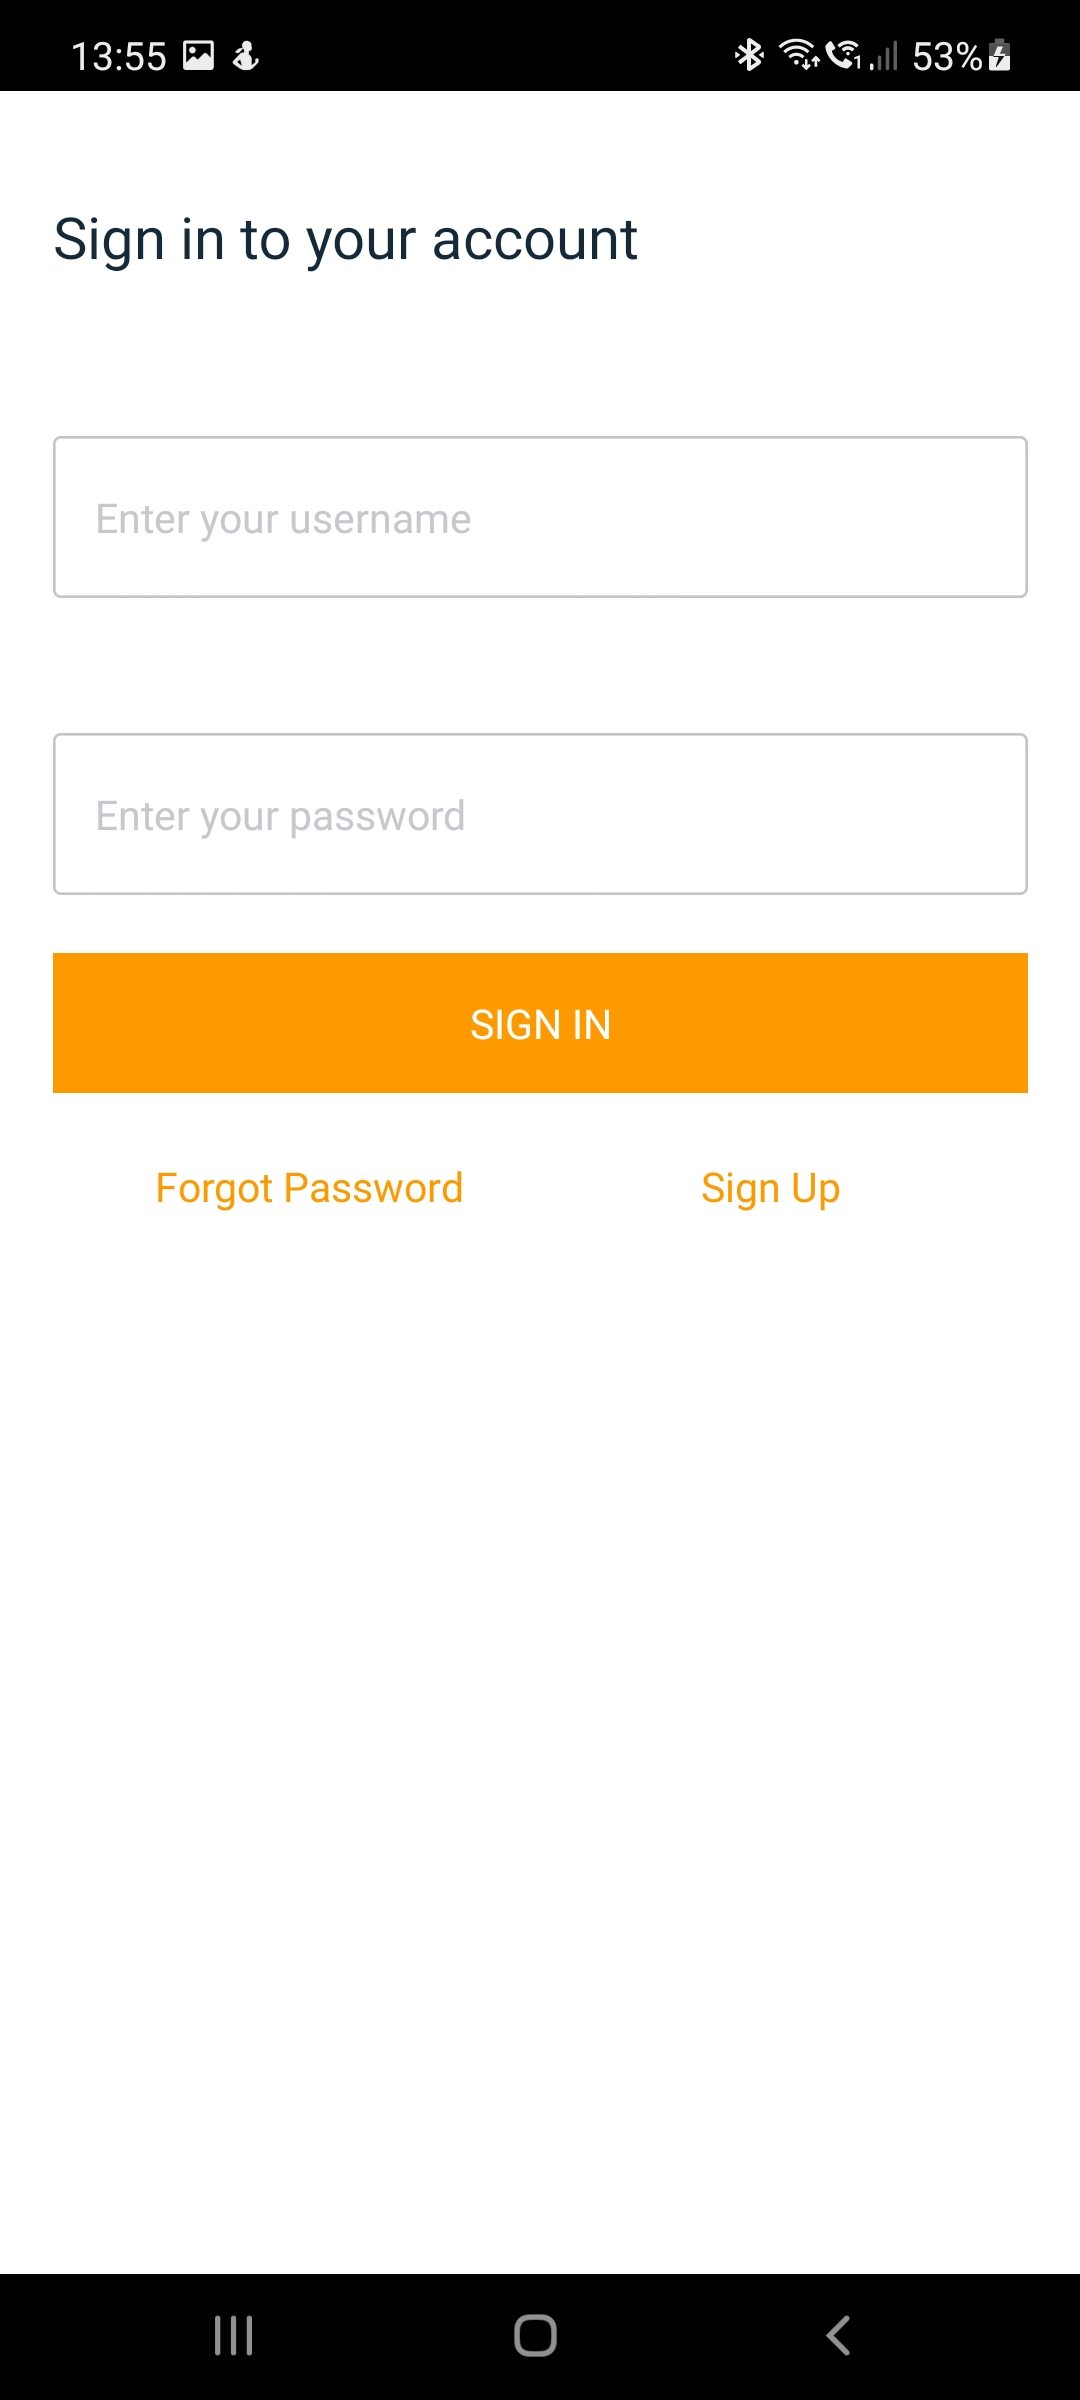
\includegraphics[width=0.6\linewidth]{img/int2.jpg}
		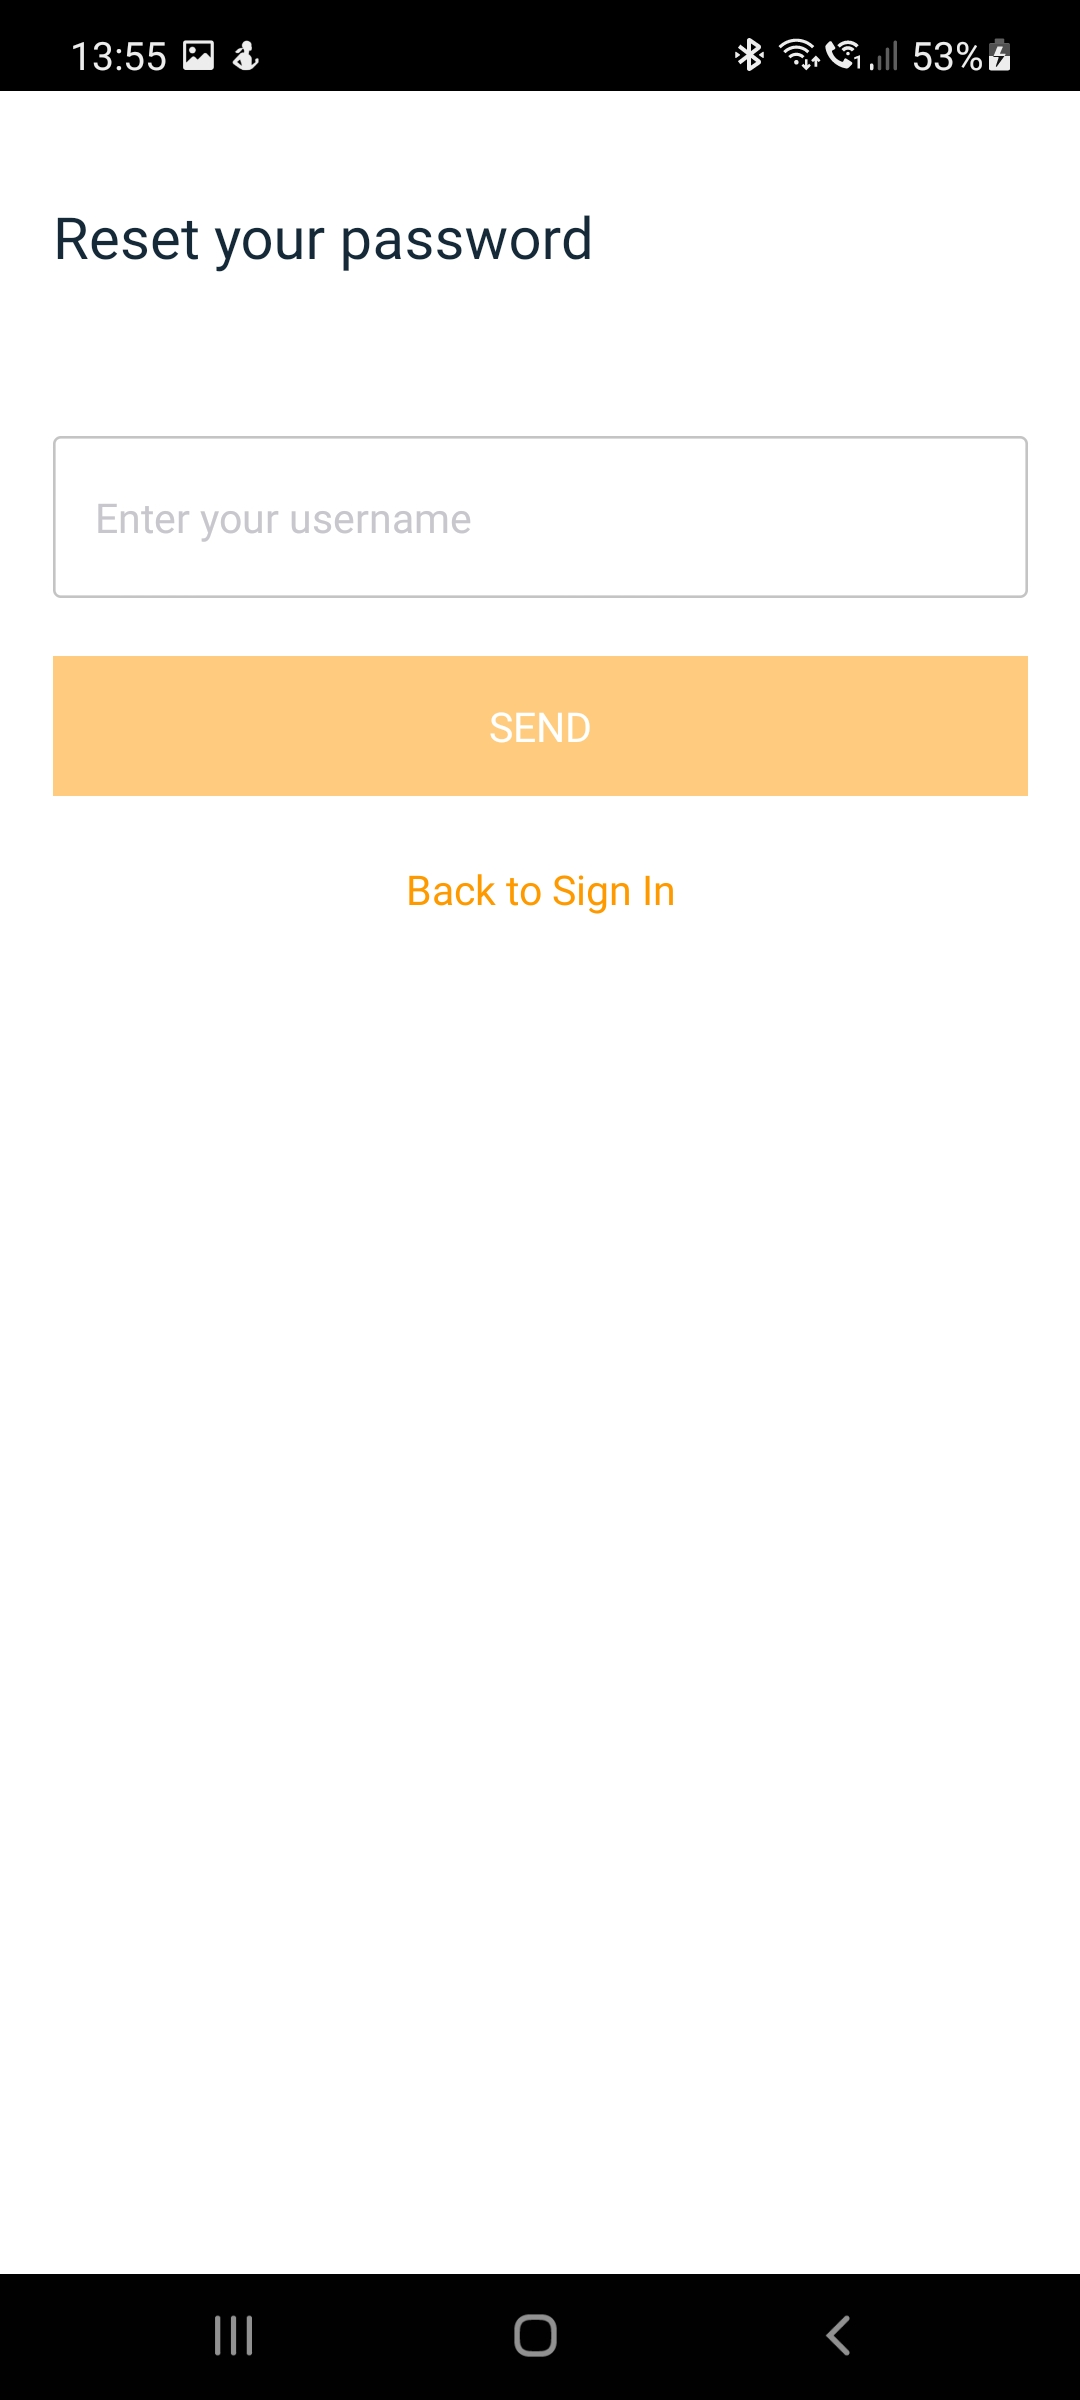
\includegraphics[width=0.6\linewidth]{img/int3.jpg}
		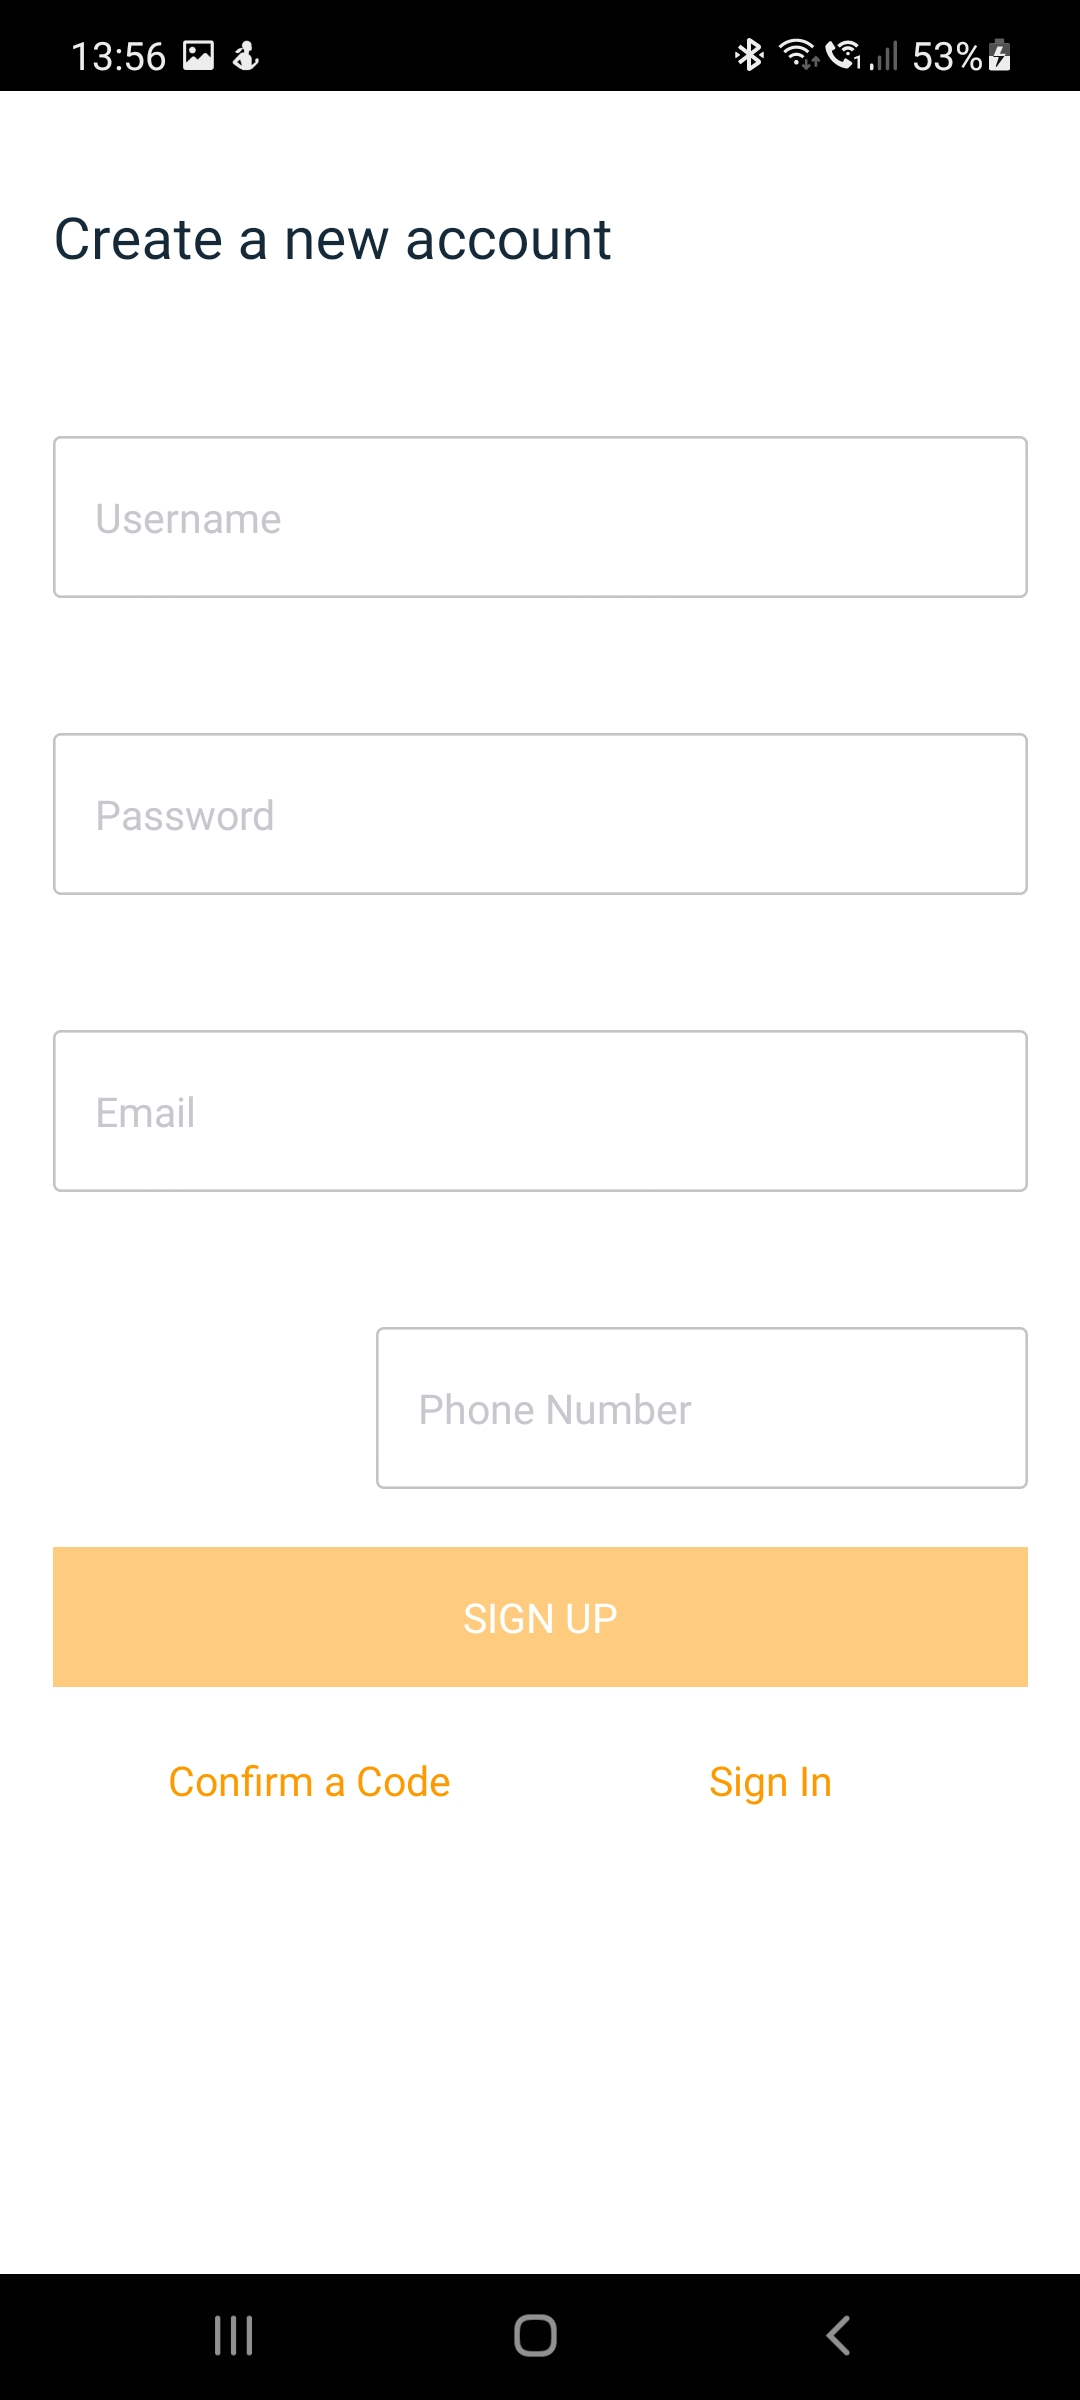
\includegraphics[width=0.6\linewidth]{img/int4.jpg}
		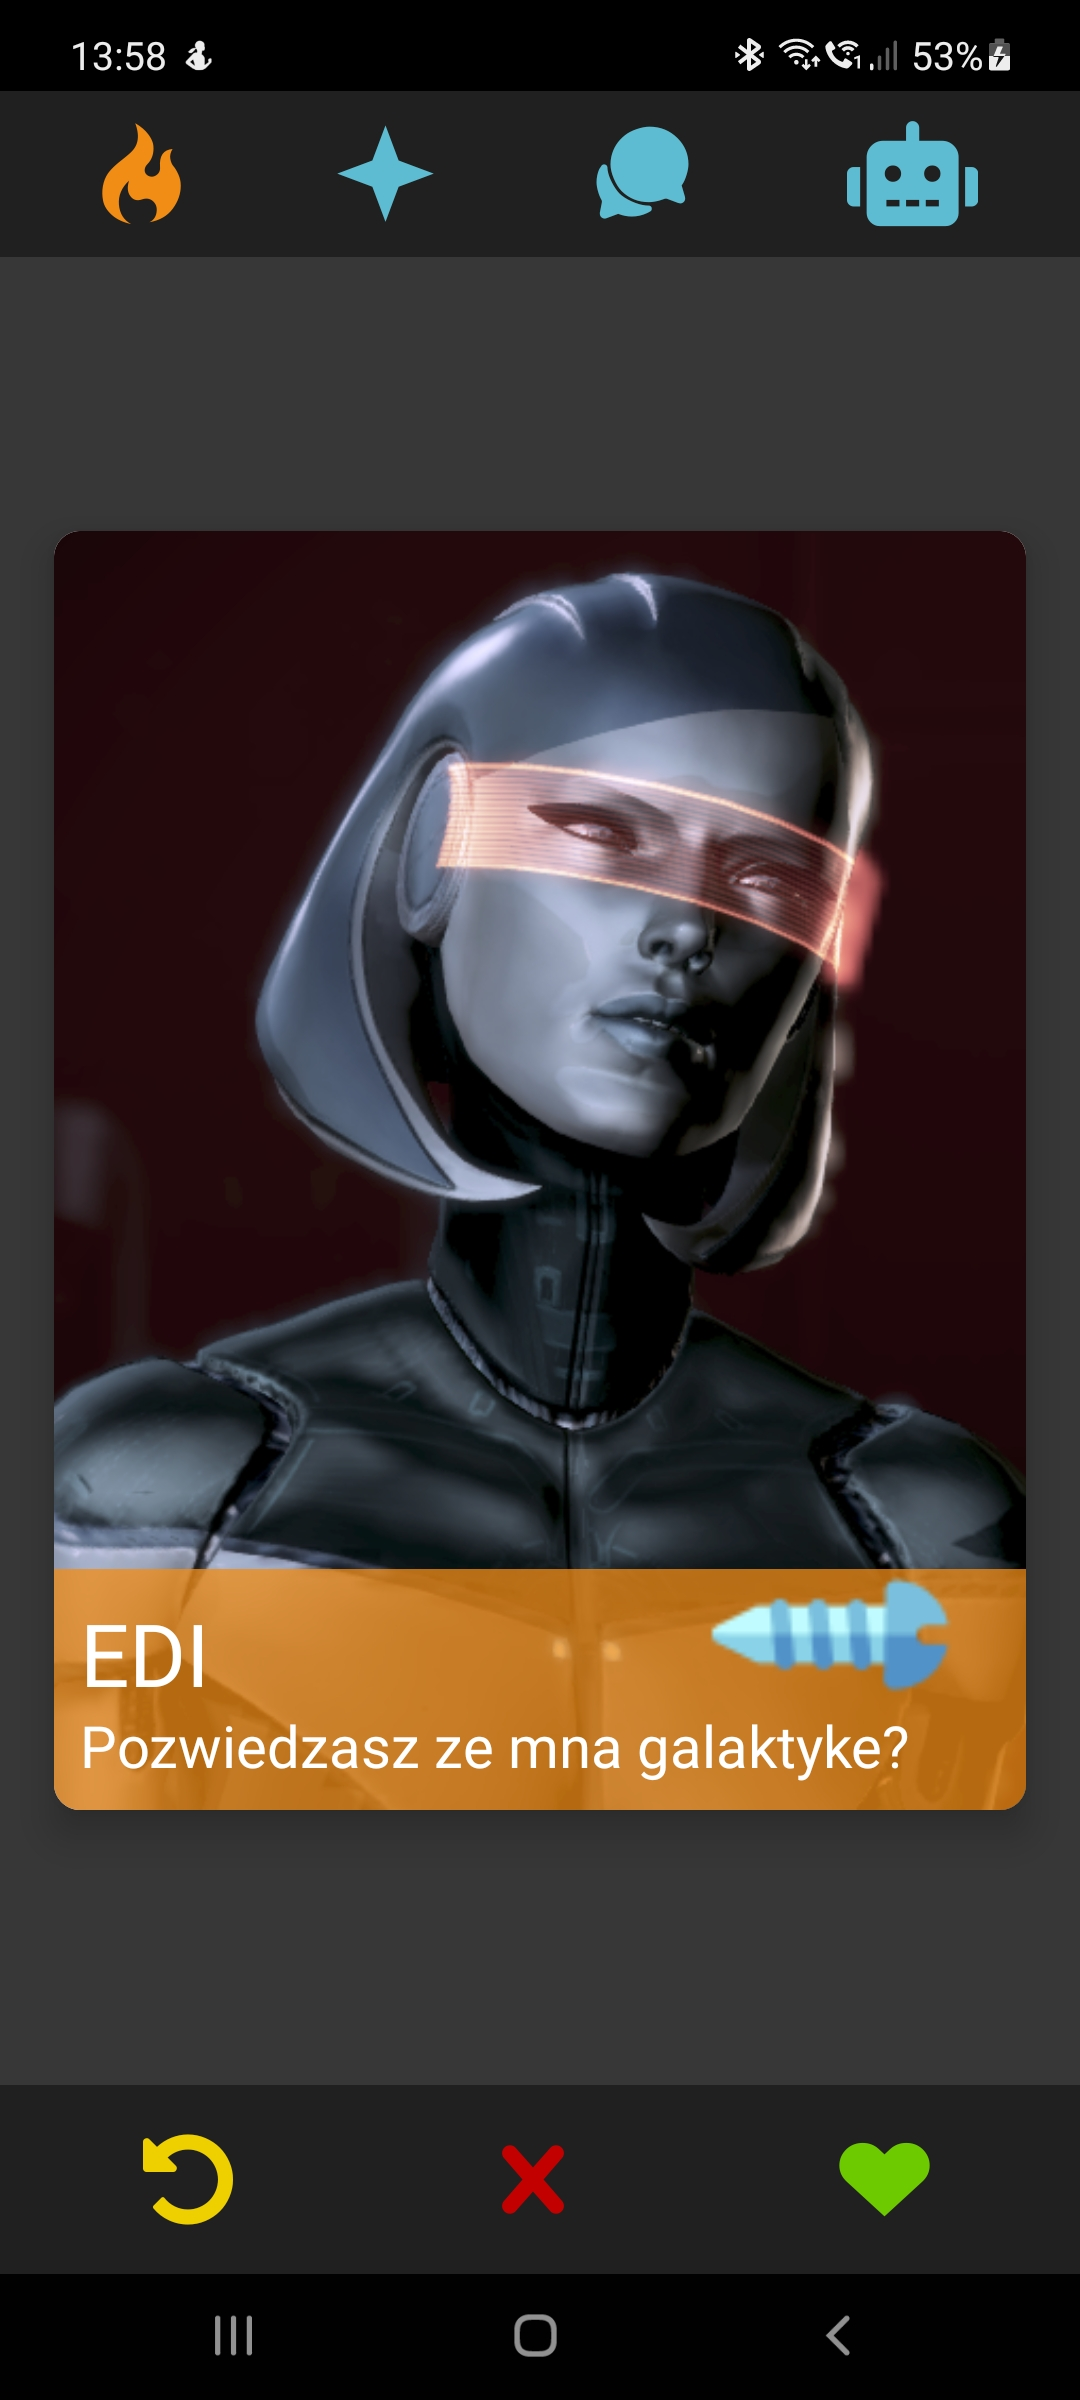
\includegraphics[width=0.6\linewidth]{img/int5.jpg}
		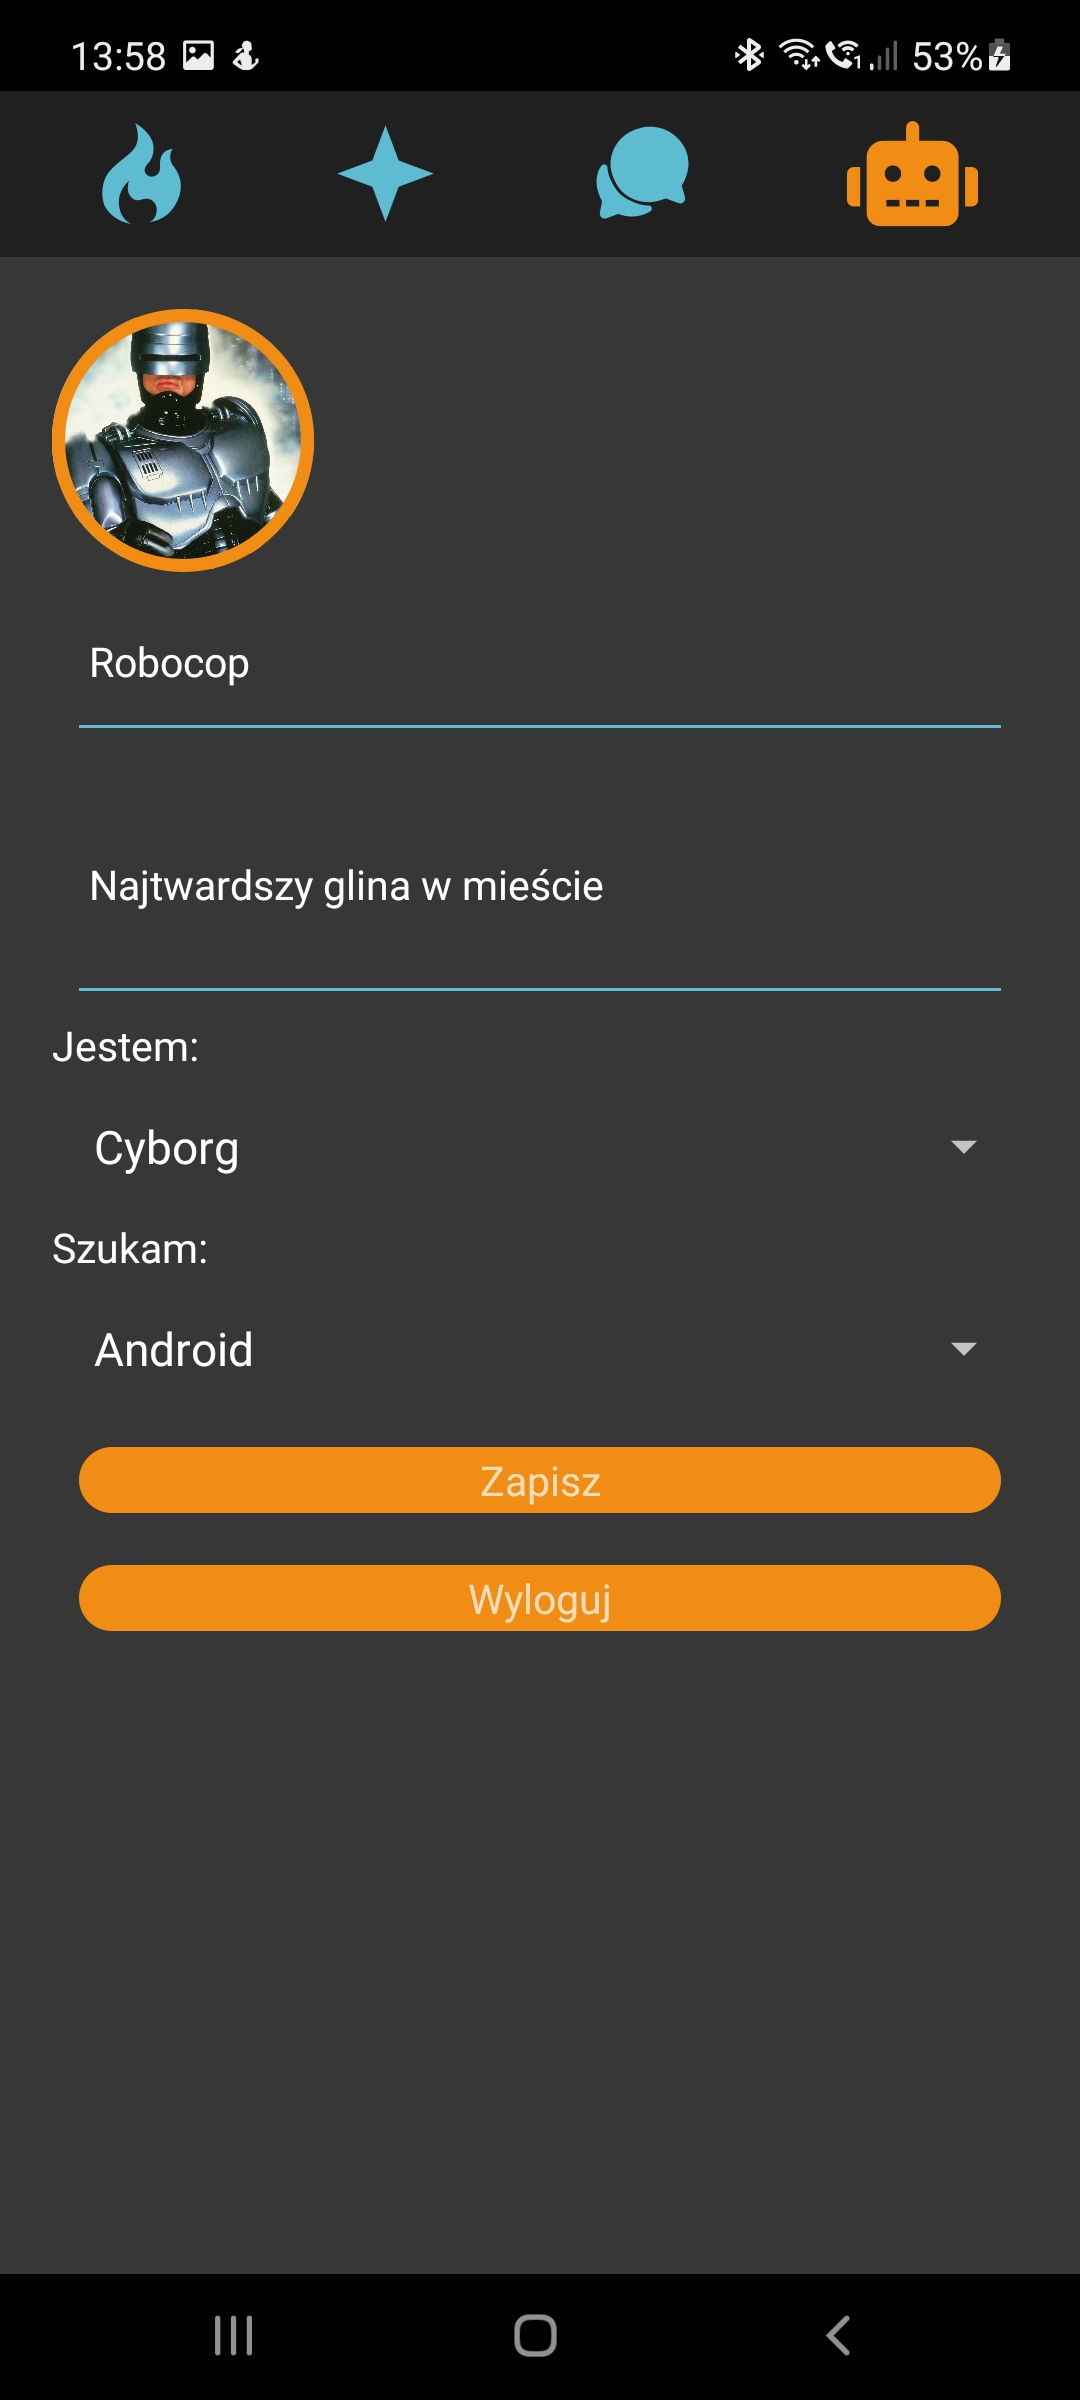
\includegraphics[width=0.6\linewidth]{img/int6.jpg}
		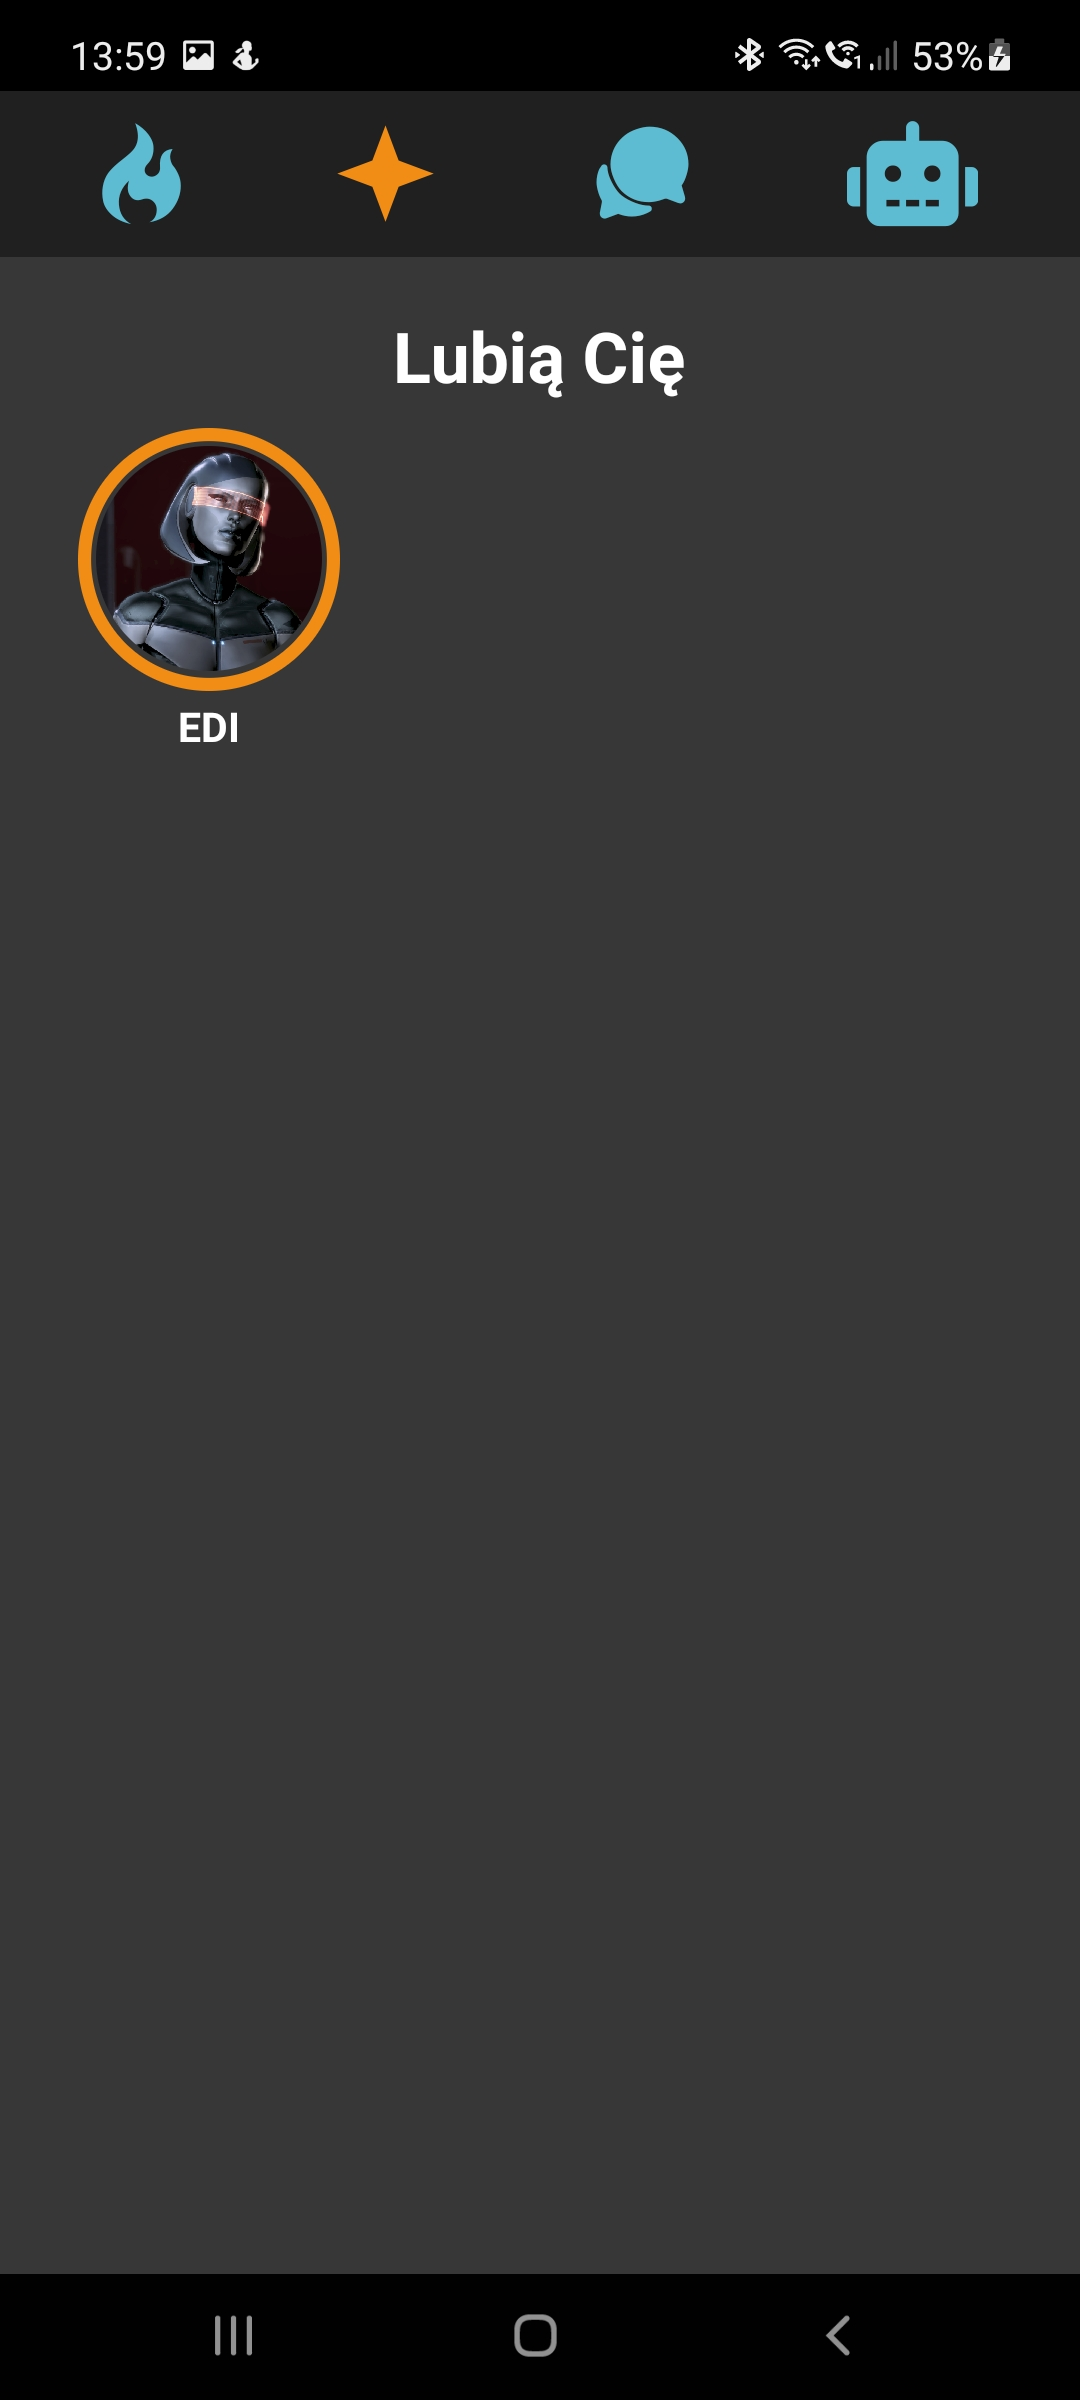
\includegraphics[width=0.6\linewidth]{img/int7.jpg}
		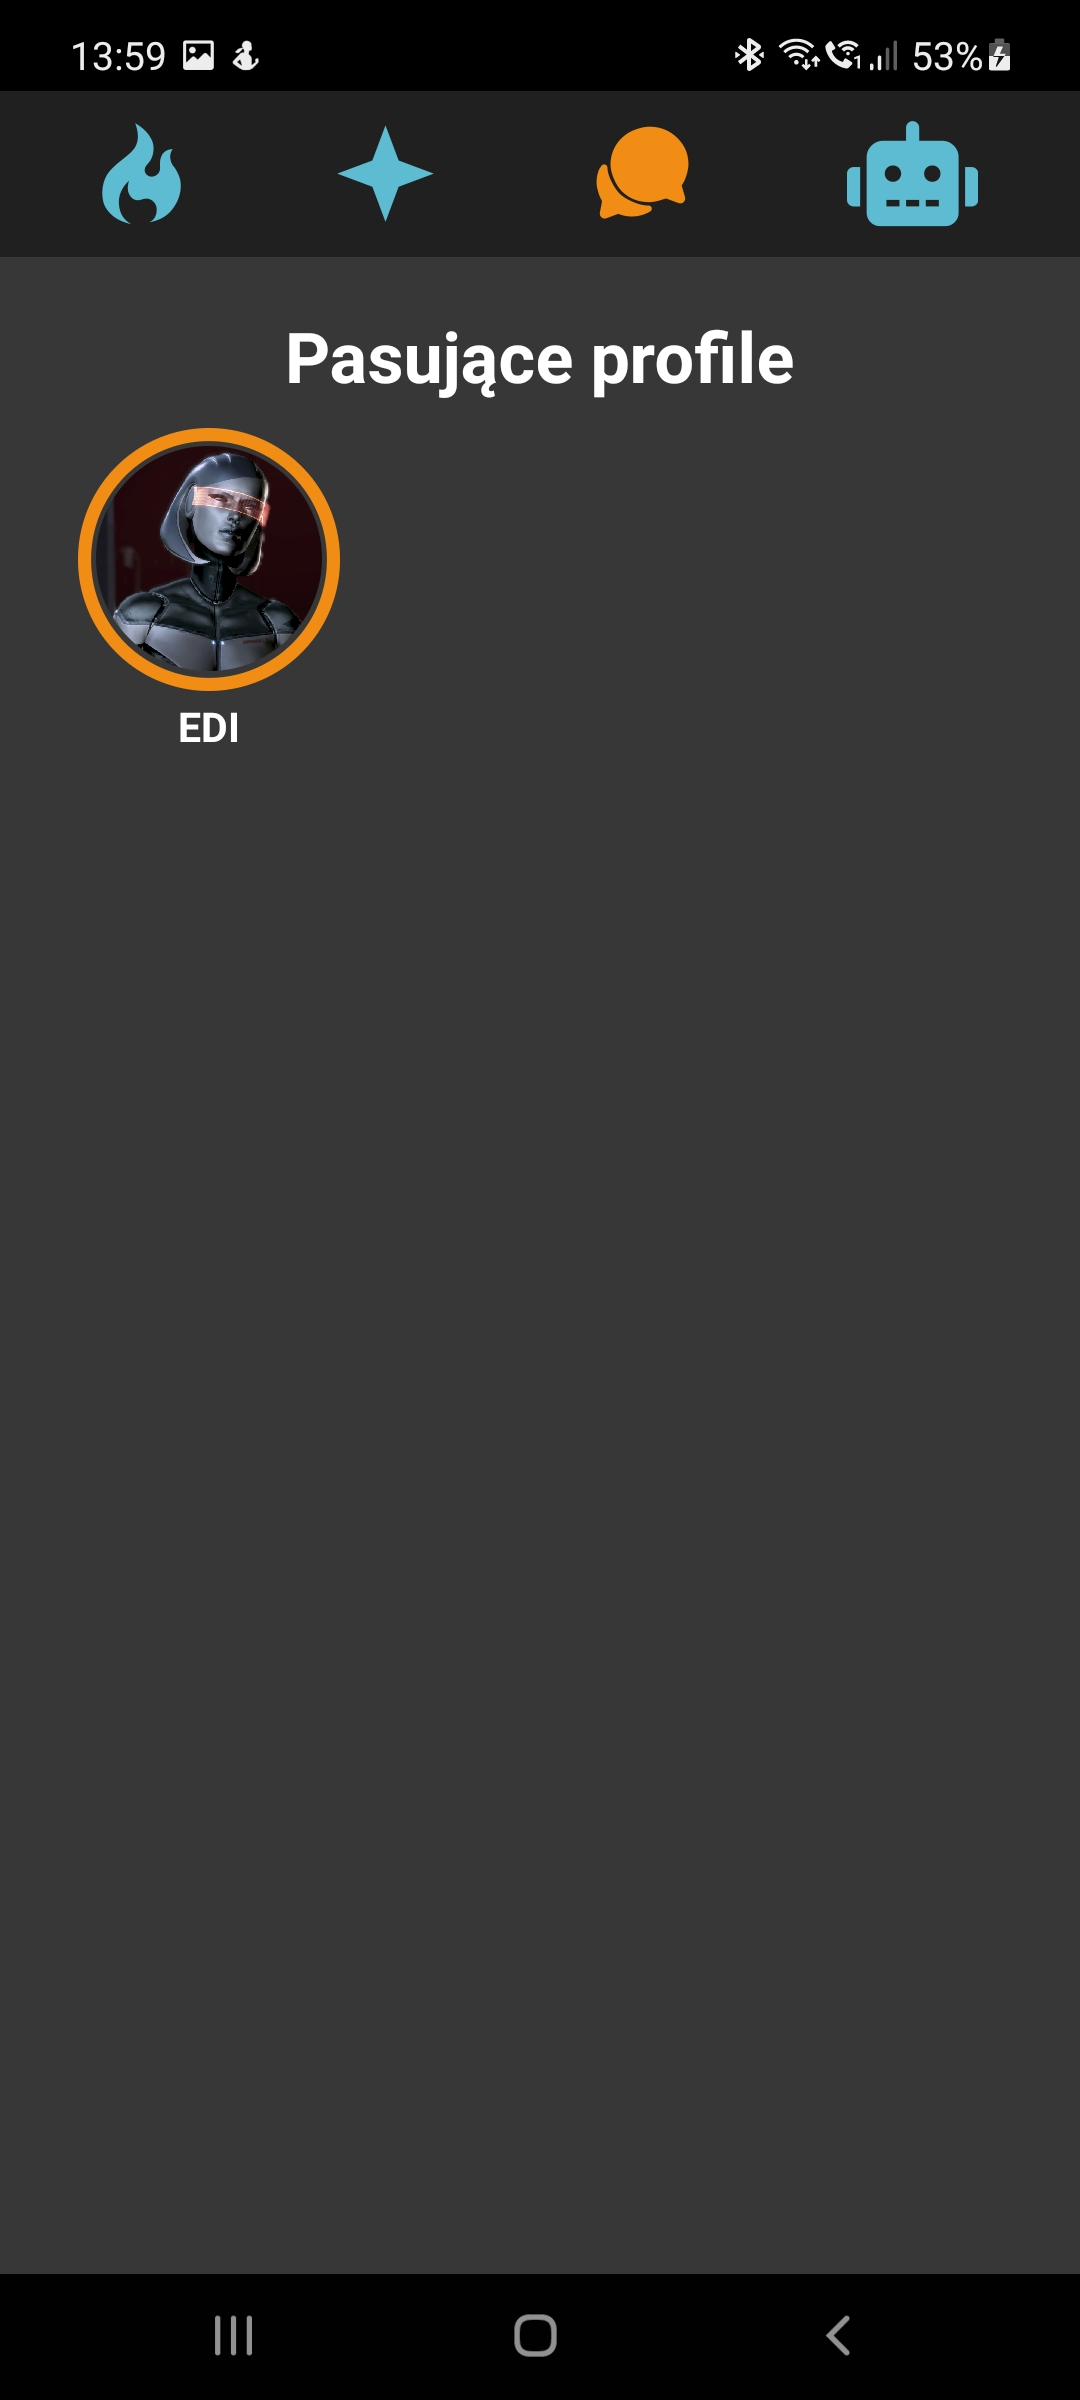
\includegraphics[width=0.6\linewidth]{img/int8.jpg}
		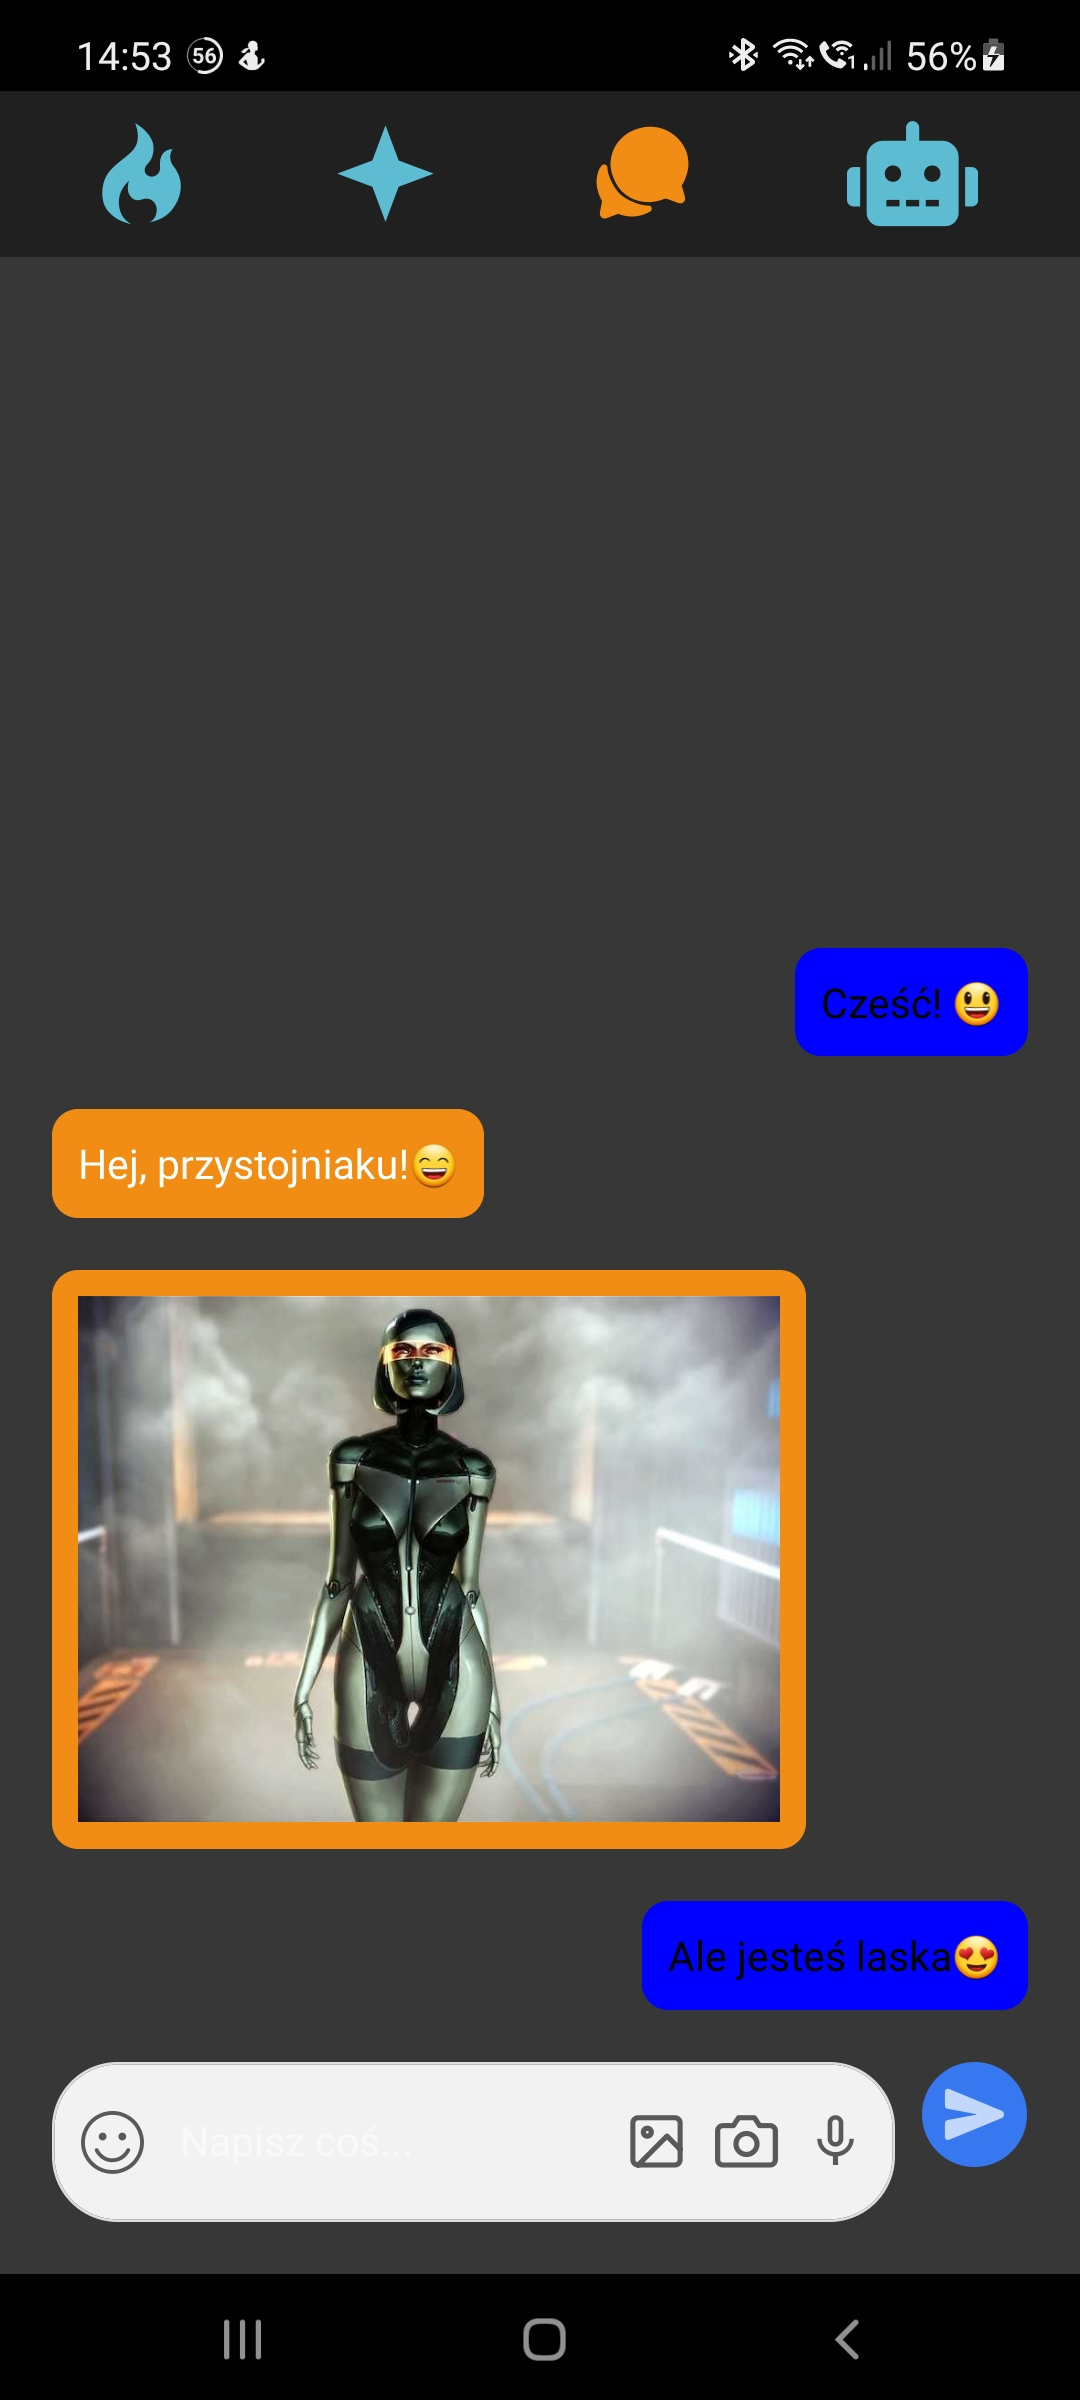
\includegraphics[width=0.6\linewidth]{img/int9.jpg}
	\end{center}
		\newpage
	\section{Instrukcja uruchomienia aplikacji}	
		\indent Przed rozpoczęciem kompilacji aplikacji potrzebne jest najpierw poprawne skonfigurowanie środowiska deweloperskiego.
		\begin{enumerate}
			\item Pobrać kod aplikacji z repozytorium projektu:\\ \url{https://github.com/MacKarp/HotScrew}
			\item Instalacja Node.js:
				\begin{itemize}
					\item Pobrać instalator Node.js w wersji 16 z strony:\\ \url{https://nodejs.org/en/download/} 
					\item Zainstalować zgodnie z instrukcjami pokazywanymi przez instalator;
				\end{itemize}
			\item Instalacja React Native:
				\begin{itemize}
					\item Zainstalować zgodnie z dokumentacją:\\ \url{https://reactnative.dev/docs/environment-setup}
					\item W katalogu HotScrew uruchomić w terminalu polecenie:
			\begin{tcolorbox}[minipage,colback=white,arc=0pt,outer arc=0pt, fontupper=\footnotesize]
				npm install							
			\end{tcolorbox}
				\end{itemize}
			\item Instalacja Amplify CLI
				\begin{itemize}
					\item Zainstalować zgodnie z dokumentacją:\\ \url{https://docs.amplify.aws/cli/start/install/}
					\item W katalogu HotScrew uruchomić w terminalu polecenie: 
					\begin{tcolorbox}[minipage,colback=white,arc=0pt,outer arc=0pt, fontupper=\footnotesize]
						amplify push
					\end{tcolorbox}
				\end{itemize}
		\end{enumerate}
		Gdy środowisko zostanie poprawnie skonfigurowane aplikację można uruchomić w emulatorze Androida przy pomocy polecenia terminala:
		\begin{tcolorbox}[minipage,colback=white,arc=0pt,outer arc=0pt, fontupper=\footnotesize]
			npx react-native run-android
		\end{tcolorbox}
		Aby skompilować aplikację dla systemu Android należy w katalogu:
		\begin{tcolorbox}[minipage,colback=white,arc=0pt,outer arc=0pt, fontupper=\footnotesize]
			HotScrew\/android
		\end{tcolorbox}
		Wykonać polecenie:
		\begin{tcolorbox}[minipage,colback=white,arc=0pt,outer arc=0pt, fontupper=\footnotesize]
			./gradlew assembleRelease
		\end{tcolorbox}
		Skompilowana aplikacja znajduje się w katalogu:
		\begin{tcolorbox}[minipage,colback=white,arc=0pt,outer arc=0pt, fontupper=\footnotesize]
			HotScrew/android/app/build/outputs/apk/release
		\end{tcolorbox}
		
		Plik ,,app-release.apk'' można wgrać na telefon z systemem Android a następnie na nim zainstalować i uruchomić.
	\newpage
	%wnioski projektowe
	\section{Wnioski projektowe}
	\indent  Tworzenie aplikacji mobilnej pozwoliła nam poszerzyć swoją wiedzę o nowe technologie. Projektowanie makiet aplikacji w Figmie było ciekawym doświadczeniem,
	które bardzo ułatwiło nam wizualizację interfejsu aplikacji, zgodnie stwierdziliśmy że mamy zamiar wykorzystywać je w przyszłości, ponieważ bardzo ułatwia
	prace nad frontendem aplikacji.	 
	Dużym wyzwaniem okazała się integracja aplikacji z usługą AWS Amplfy spowodowany niedawnymi dosyć sporymi zmianami w API, co spowodowało że duża część materiałów
	dostępnych w internecie były przestarzałe. Dodatkowo dokumentacja AWS SDK również nie została jeszcze w całości zaktualizowana lub brakuje części instrukcji
	migracji do nowej wersji API. Kolejnym problemem, który się pojawił było zrobienie CI/CD, które by automatycznie budowała i podpisywała aplikację Androida,
	okazało się że nie da się wygenerować wymaganych plików konfiguracyjnych dla AWS SDK przy użyciu GitHub Actions. Możliwe jest to tylko wykorzystując cały
	pipline AWS(wraz z repozytorium kodu) -  co ze względów na wymagania projektowe - było niemożliwe.
	
\end{document}
